% This is "sig-alternate.tex" V2.1 April 2013
% This file should be compiled with V2.5 of "sig-alternate.cls" May 2012
%
% This example file demonstrates the use of the 'sig-alternate.cls'
% V2.5 LaTeX2e document class file. It is for those submitting
% articles to ACM Conference Proceedings WHO DO NOT WISH TO
% STRICTLY ADHERE TO THE SIGS (PUBS-BOARD-ENDORSED) STYLE.
% The 'sig-alternate.cls' file will produce a similar-looking,
% albeit, 'tighter' paper resulting in, invariably, fewer pages.
%
% ----------------------------------------------------------------------------------------------------------------
% This .tex file (and associated .cls V2.5) produces:
%       1) The Permission Statement
%       2) The Conference (location) Info information
%       3) The Copyright Line with ACM data
%       4) NO page numbers
%
% as against the acm_proc_article-sp.cls file which
% DOES NOT produce 1) thru' 3) above.
%
% Using 'sig-alternate.cls' you have control, however, from within
% the source .tex file, over both the CopyrightYear
% (defaulted to 200X) and the ACM Copyright Data
% (defaulted to X-XXXXX-XX-X/XX/XX).
% e.g.
% \CopyrightYear{2007} will cause 2007 to appear in the copyright line.
% \crdata{0-12345-67-8/90/12} will cause 0-12345-67-8/90/12 to appear in the copyright line.
%
% ---------------------------------------------------------------------------------------------------------------
% This .tex source is an example which *does* use
% the .bib file (from which the .bbl file % is produced).
% REMEMBER HOWEVER: After having produced the .bbl file,
% and prior to final submission, you *NEED* to 'insert'
% your .bbl file into your source .tex file so as to provide
% ONE 'self-contained' source file.
%
% ================= IF YOU HAVE QUESTIONS =======================
% Questions regarding the SIGS styles, SIGS policies and
% procedures, Conferences etc. should be sent to
% Adrienne Griscti (griscti@acm.org)
%
% Technical questions _only_ to
% Gerald Murray (murray@hq.acm.org)
% ===============================================================
%
% For tracking purposes - this is V2.0 - May 2012

\documentclass{acm_proc_article-sp}
\usepackage{color}

\begin{document}

% Copyright
%\setcopyright{acmcopyright}
%\setcopyright{acmlicensed}
%\setcopyright{rightsretained}
%\setcopyright{usgov}
%\setcopyright{usgovmixed}
%\setcopyright{cagov}
%\setcopyright{cagovmixed}


% --- End of Author Metadata ---

\title{Final Project Proposal}
%\subtitle{[Extended Abstract]
%
% You need the command \numberofauthors to handle the 'placement
% and alignment' of the authors beneath the title.
%
% For aesthetic reasons, we recommend 'three authors at a time'
% i.e. three 'name/affiliation blocks' be placed beneath the title.
%
% NOTE: You are NOT restricted in how many 'rows' of
% "name/affiliations" may appear. We just ask that you restrict
% the number of 'columns' to three.
%
% Because of the available 'opening page real-estate'
% we ask you to refrain from putting more than six authors
% (two rows with three columns) beneath the article title.
% More than six makes the first-page appear very cluttered indeed.
%
% Use the \alignauthor commands to handle the names
% and affiliations for an 'aesthetic maximum' of six authors.
% Add names, affiliations, addresses for
% the seventh etc. author(s) as the argument for the
% \additionalauthors command.
% These 'additional authors' will be output/set for you
% without further effort on your part as the last section in
% the body of your article BEFORE References or any Appendices.

\numberofauthors{1} %  in this sample file, there are a *total*
% of EIGHT authors. SIX appear on the 'first-page' (for formatting
% reasons) and the remaining two appear in the \additionalauthors section.
%
\author{
% You can go ahead and credit any number of authors here,
% e.g. one 'row of three' or two rows (consisting of one row of three
% and a second row of one, two or three).
%
% The command \alignauthor (no curly braces needed) should
% precede each author name, affiliation/snail-mail address and
% e-mail address. Additionally, tag each line of
% affiliation/address with \affaddr, and tag the
% e-mail address with \email.
%
% 1st. author
\alignauthor
Caitlin Ross, Noah Wolfe\\
       \affaddr{Computer Science Department \\ Rensselaer Polytechnic Institute}\\
       \email{(rossc3, wolfen) @rpi.edu}
% 2nd. author
}
% There's nothing stopping you putting the seventh, eighth, etc.
% author on the opening page (as the 'third row') but we ask,
% for aesthetic reasons that you place these 'additional authors'
% in the \additional authors block, viz.
%\additionalauthors{Additional authors: John Smith (The Th{\o}rv{\"a}ld Group,
%email: {\texttt{jsmith@affiliation.org}}) and Julius P.~Kumquat
%(The Kumquat Consortium, email: {\texttt{jpkumquat@consortium.net}}).}
\date{30 July 1999}
% Just remember to make sure that the TOTAL number of authors
% is the number that will appear on the first page PLUS the
% number that will appear in the \additionalauthors section.

\maketitle
%\begin{abstract}
%
%\end{abstract}
%

%
% The code below should be generated by the tool at
% http://dl.acm.org/ccs.cfm
% Please copy and paste the code instead of the example below. 
%


%
% End generated code
%

%
%  Use this command to print the description
%
%\printccsdesc

% We no longer use \terms command
%\terms{Theory}

%\keywords{ACM proceedings; \LaTeX; text tagging}

\section{Introduction}
For the final project, we propose to create an interactive interface for exploring simulation level data of parallel simulations.  We use the Rensselaer Optimistic Simulation System (ROSS), which is a massively parallel discrete-event simulator that can process billions of events per second \cite{Holder}, \cite{Bauer}.  With event-driven simulation, there are logical processes (LPs) that represents entities being simulated (e.g., a router in a network) and each LP has a set of events defined that it sends to and receives from other LPs in the system.  For parallel execution, the LPs are mapped to the different processing elements (PEs). We use an optimistic parallel protocol for our ROSS simulations.  In optimistic execution, PEs process their assigned events without global synchronization with other PEs.  When a LP determines that it has processed an event out of timestamp order, it rolls back events in order to re-execute the events in the correct order.

For our visualizations, we will be looking at the performance of the Dragonfly and Slim Fly network models that were developed for ROSS.  
\color{red}Noah, can you add some details on the models here? \color{black}

Our target audience for these visualizations is PDES developers, especially anyone doing their development with ROSS.  The research questions we want to be answered by our visualization are:
\begin{itemize}
\item \textbf{How can we boost the performance of the simulation?} The visualization should help to highlight areas where improvement is needed to boost performance.
\item  \textbf{How does the performance of the dragonfly and slim fly models differ?}  For this question, the visualization should show which simulation-level statistics are associated with these performance differences.
\end{itemize}

\color{red}Hypothesis for these questions with our data?\color{black}

\section{Extensions to ROSS}
The Dragonfly and Slim Fly models have already been developed, but ROSS does not currently have the ability to collect simulator level statistics for given time intervals.  To complete the visualizations for this project, we are adding extensions to ROSS for the statistics collection.  We will be collecting the number of remote sends, receives,  forward events, reverse events, and rollbacks.  The data can be collected for time intervals specified by the user.  Also, the data will be collected on a LP basis and all of the data for LPs on a given PE can be combined to visualize the data on a PE basis.  

\section{User Interface}
\begin{figure*}[t]
\centering
   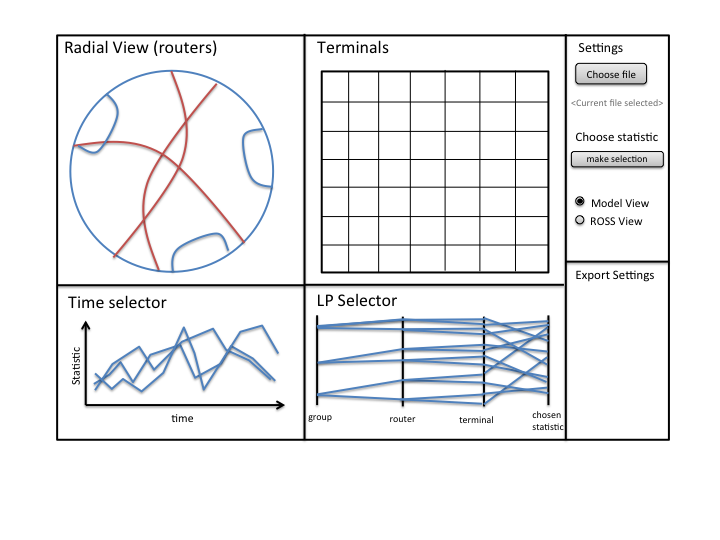
\includegraphics[width=6.5in, clip=true, trim=0 1in 0 0]{../figures/gui-diagram/Slide1.png}
\caption{Model View}
\label{model-view}
\end{figure*}

\begin{figure*}[t]
\centering
   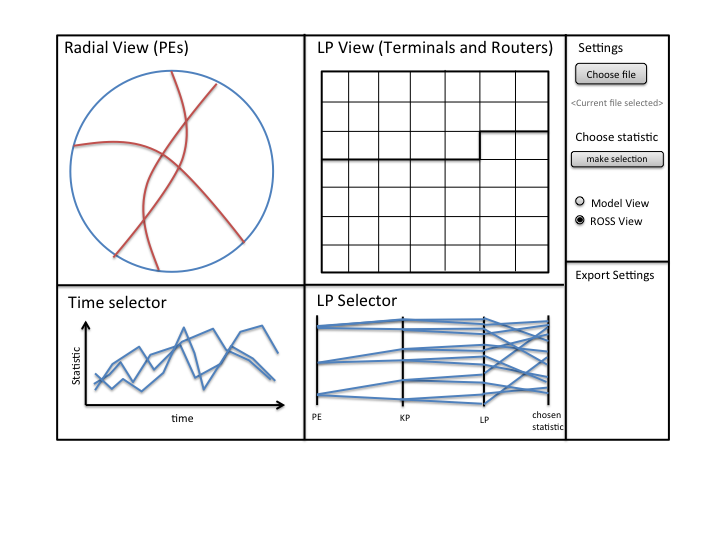
\includegraphics[width=6.5in, clip=true, trim=0 1in 0 0]{../figures/gui-diagram/Slide2.png}
\caption{ROSS View}
\label{ross-view}
\end{figure*}

We plan to make this interface available on the web using D3.  Our interface will have two main views: a Model View and a ROSS View.  For both views, there is a settings area on the right side of the screen.  Here a file can be selected to load in the data.  You can also choose from a drop down box which statistic to view data for.  Then the user can select either of the two views.  Below that is an export settings area.  We haven't decided on the final settings to be allowed, but we plan to allow the user to export the entire workspace (i.e., all four graphs) as an image as well as the ability to save each graph as its own image file.  

The workspace of the GUI contains four different interactive visualizations that change depending on whether the Model View or the ROSS View is chosen.  This part of the interface was inspired by Cheng et al.~\cite{cheng}.  In their paper, they describe an interactive interface that visualizes the traffic over a 5D torus network.  They have a radial diagram that shows network traffic, a parallel coordinates graph to allow for node selection, and a stream graph which shows some property of the network over time as a streamgraph.  The streamgraph also allows the user to select a point in time which updates the view in the radial diagram.  Similarly nodes can be selected in the parallel coordinates to update the radial diagram.

For the Model View, which is shown in Figure~\ref{model-view}, we have a radial diagram in the upper left corner of the workspace.  This will have routers placed on the circle, with edges representing the links between routers.  Currently the red edges show global connections among the routers, while the blue edges show local connections.  For the actual interface, we have two ideas we are considering for the edge colors.  One way is to keep the different colors for the two different connections and vary the saturation of the color based on the values of the statistic being measured.  The other way is to use the same sequential color scheme for both types of links.  In the ROSS view, shown in Figure~\ref{ross-view}, the PEs will be placed on the circle, with connections between PEs representing the communication between PEs during simulation.  Based on the mappings of LPs to PEs in both network models, it is possible for any PE to communicate with all other PEs, but we will use a similar color scheme as what is used in the Model View.  Particularly for large-scale runs (for either the ROSS or Model views), we will probably need to use hierarchical edge bundling~\cite{jia} in order to make the diagram easier to read and understand.  

The LP selector is shown in the bottom right of the workspace area.  This is a parallel coordinates graph.  For the Model View, the axes are for groups, routers, terminals, and the chosen statistic.  For the ROSS view, the axes are PEs, KPs, LPs, and the chosen statistic.  We are also considering having additional axes shown for all statistics that are being measured, in order to provide additional context.  Brushing~\cite{hauser} can be used on the axes to select a subset of the data, which will also update the routers/PEs being shown in the radial view.  

We will also have a time selector, shown in the bottom left corner of the workspace, although we are currently planning to use line graphs instead of streamgraphs used in~\cite{cheng}.  The statistic being viewed can be selected in settings and will contain data for all of the LPs.  This graph should look similar for both the Model and ROSS views.  The data shown on this graph can also be updated based on the choices made in the LP Selector graph.  

Finally, we have a fourth visualization, which is placed in the upper right corner of the workspace.  This allows for viewing some aspects of the data in more detail.  In the Model View, this is a grid of terminals that are connected to the routers.  The terminals will be colored as a heat map based on the values of the statistic being viewed.  For the ROSS View, squares in the grid can represent either terminals or routers, which will be separated by a thicker border (as seen in Figure~\ref{ross-view}).  The terminals and/or routers shown here can be updated by all of the previously described visualizations in order to be able to view only certain entities.  



\section{Timeline}
The tasks we need to accomplish for this project are as follows:
\begin{itemize}
\item Finish development of the ROSS statistics collection
\item Perform runs of network models with statistics collection enabled
\item Create the GUI, focusing first on the radial view and the LP selector
\item Add the time selector and Terminal/Router grid
\end{itemize}

Our plan is to be able to complete all of these items and have a complete visualization for the Model View.  If time allows, we then plan to make the necessary adjustments for the ROSS view.  Caitlin is currently working on the implementation for statistics collection in ROSS as part of her research and parallel computing class project.  Some basic stats collection has already been implemented, but it is only being collected on a PE basis currently.  Noah has the most experience with the network models being studied, so he will perform the runs to collect the data after the implementation for statistics collection is done.  We will both work on development of the GUI.  We have some Javascript code from our previous class homeworks that will help us to implement the GUI.  

\section{Risks and Limitations}
There are several risks involved in being able to fully complete the interface we have discussed here.  One is that the collection of stats on the LP basis (as opposed to PEs) may not be finished in time, so that will have a large effect on the final product.  Ideally we'd like to do massively parallel runs on the Blue Gene/Q for data collection for our visualization, so we could run into some issues in dealing with large-scale data collection.  Even if we are unable to get all of the data we are currently anticipating, we believe that we can have enough development done on the visualization interface done in order to produce some helpful visualizations in the time frame of the class project.

One final risk is that neither one of us is particularly experienced with Javascript and we've had some difficulty with certain features of D3 on previous assignments.   This could potentially eat up a lot of time and we may not be able to complete the fully interactive interface.  For this, we plan to get all four visualizations done and try to finish as much of the interactive features between the visualizations as possible.  
    

\section{Feedback from other students}
Together we received three comments from classmates on our project idea.  Two comments basically stated that they thought this would be a really helpful system for debugging and optimizing simulations.  A third student asked if all of the diagrams would be integrated into one application and whether the visualizations would be created in situ or post hoc.  Here we focus on post hoc processing, but future work for our research group involves enabling in situ visualization for large-scale simulations.  

%\begin{itemize}
%\item I think creating some tool to help visualize what is going on ?behind the curtains? will help tremendously when debugging or optimizing the simulation. I dont know much about collecting data from simulations or how it is structured so I cannot give any suggestions on how to go about it.
%\item Would all of these diagrams be integrated into one application with an overall control flow, or would they be separated tools with separated controls?  Would they be updated in real time, or calculated and displayed in total after calculation has completed?  If the former, how large do you anticipate the slowdown will be?
%\item I?m in Carother?s parallel computing class, and I like the idea of doing a visualization for a supercomputer level simulation. Simulations can yield a lot of mean- ingful data that isn?t just results, and a visualization to look at that can be really useful. Especially on a supercomputer, where performance is really the only thing that matters, a visualization can show not just
%how to make the program/simulation better, but could show a shortcoming of the whole system.
%\end{itemize}



%\section{Conclusions}

%\end{document}  % This is where a 'short' article might terminate

%ACKNOWLEDGMENTS are optional
%\section{Acknowledgments}

%
% The following two commands are all you need in the
% initial runs of your .tex file to
% produce the bibliography for the citations in your paper.
\bibliographystyle{abbrv}
\bibliography{proposal}  % sigproc.bib is the name of the Bibliography in this case
% You must have a proper ".bib" file
%  and remember to run:
% latex bibtex latex latex
% to resolve all references
%
% ACM needs 'a single self-contained file'!
%
%APPENDICES are optional
%\balancecolumns


%\balancecolumns % GM June 2007
% That's all folks!
\end{document}
